\newpage
\section{Root functional modelling} \label{sec:functional}

Root growth is strongly influenced by pedo-climatic conditions, and plant internal state. CPlantBox offers 'build in' ways to develop such models, see \cite{schnepf2018crootbox}. 

CPlantBox is a bottom up model were root growth is first defined under perfect conditions. Adding mechanisms to take environmental conditions into account will alter the root system development by impeding root growth, and by changing soil allocation by roots due to root tropism and due to altered branching patterns.

In this section we assume static soil conditions, and demonstrate the predefined ways how the soil can affect root growth.
Dynamic soil conditions are described in the following Section \ref{s:coupling}. 

Implemented root responses are the change in direction of the growing root tip, as described in previous Section \ref{sec:tropism}.
Further root responses are 
\begin{itemize}
 \item scaling of the elongation rate 
 \item change of insertion angle
 \item change of lateral emergence probability
\end{itemize}

\subsection{Scaling the elongation rate} \label{sec:elongation}

Root elongation rate is influenced by soil properties such as water content, temperature, soil density, solutes, and many more. Regarding the processes that are investigated, various models can be applied. In CPlantBox the elongation rate is scaled with no predefined interpretation, i.e. we have to define a elongation rate scaling, which is dependent on such soil properties. The following example defines two compartments (one left, one right), where we change this scaling, and then analyse the results. The same procedure will be used in Example \ref{sec:insertion_angle} and \ref{sec:branching}.

\lstinputlisting[firstline=1, language=Python, caption=Example 5a]{../../examples/python/example5a_elongation.py}

\begin{itemize}

\item[7-10] Creates the root system and opens the parameter file.

\item[13-17] We create a confining box with two overlapping boxes called $left$ and $right$. These geometries are used for later analysis.

\item[20-24] We define static soil properties using SDF (L23, L24) as we did in Section \ref{sec:hydro}. 
The left compartment has the value $minS$, the right $maxS$, between them is a linear gradient of length $slope$. 

\item[27-31] Sets the scaling functions. L29 adjusts axial resolution and L30 tortuosity $sigma$. L31 sets the scale elongation function $f_{se}$ to the soil property (i.e. scales to $minS$ in the left, $maxS$ in the right compartment). 

\item[34-39] Initialization and simulation loop. In a dynamic setting, $soilprop$ needs to be updated in each time step (comment L38).

\item[42-50] Analysis the root length in the left and right compartment. With parameters $minS$ and $slope$ only approximately $21\%$ are located in the left compartment.

\item[53, 54] Writes the results for Paraview visualization (see Figure \ref{fig:elongation}).

\item[57] A vtk simulation of root lengths. Press 'y' to obtain a x-z view of the root system to better see the effect. 

\end{itemize}
 
Next, we give a short layout, how the code would look like, if we take measured data (e.g. density versus depth), and include it in the simulation. 

\lstinputlisting[firstline=1, language=Python, caption=Example 5b]{../../examples/python/example5b_scaleelongation.py}

\begin{itemize}

\item[12-16] In L12 an EquidistantGrid1D is created, which is a specialisation from SoilLookUp (in soil.hh). It represents a 1D grid from 0 cm to -100 cm as soil with 100 layers. Additionally scalar data are attached to the grid, L13, L14 we create example soil strength data. From this data we calculate the elongation scales (L15), and set it as grid data (L16). 

\item[L17, L18] Retrieve the elongation scale data at two points. The data is given per layer, no data interpolation is performed.

\item[20, 21] Sets the elongation scaling function to all root types.

\item[25-32] Subsection \ref{ssec:animation} explains how to make an animation in Paraview. Here we use another (slower) approach to create the animation (and a preview) directly in vtk. For this we create an AnimateRoots object (L26), choose the domain size, and start the rendering (L32). 

\item[34-50] Simulation loop. If soil strength changes, the elongation scales must be calculated again (L32), and attached to the grid (L35). The frames of the animations are written in L50. While the approach is convenient, it is rather slow since for each frame a SegmentAnalyser object is created and rendered from scratch which is not feasible for large root systems. 

\item[52,53] Exports results as vtp, and creates a vtk plot. The effect of the dense layer can hardy be seen in the results (between -10 and -15 cm depth, laterals will be shorter). But the created animation reveals the effect (see exported video example5b.ogv). 

\end{itemize}

\begin{figure}
\centering
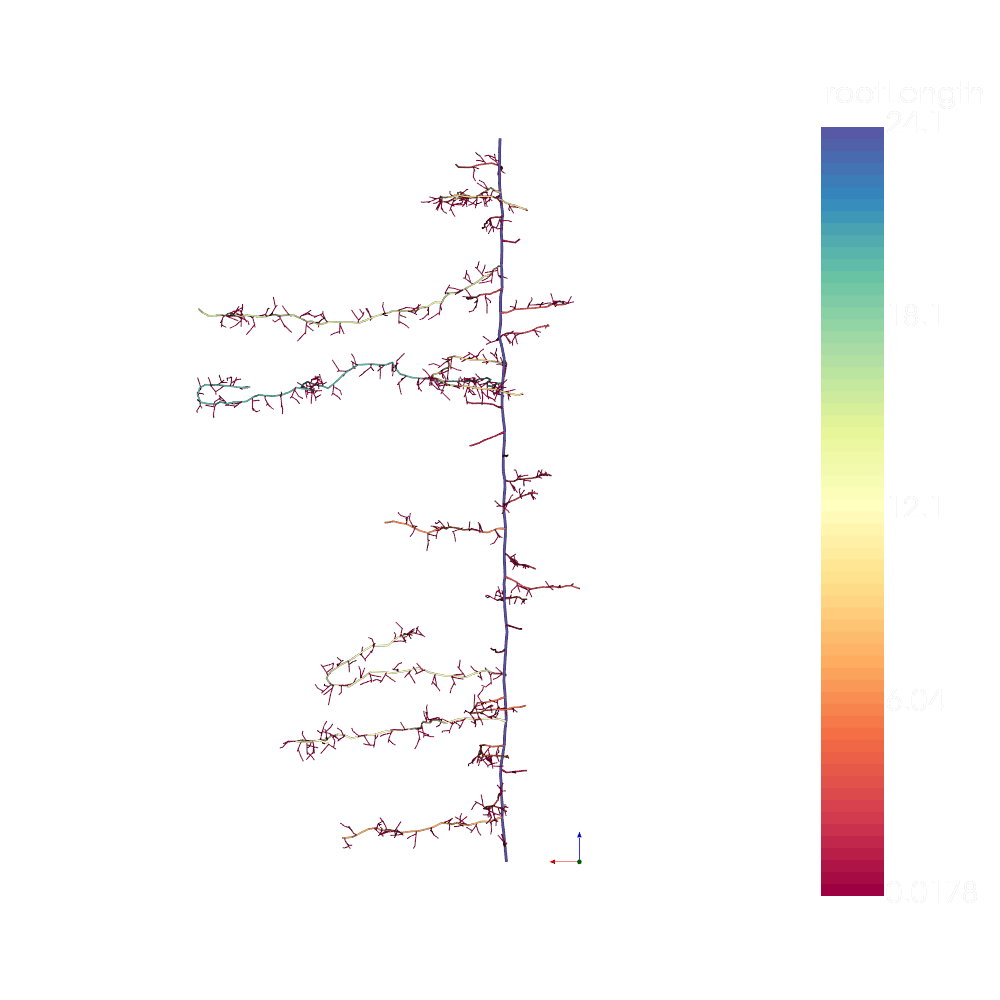
\includegraphics[width=0.5\textwidth]{example5a.png}
\caption{Root elongation rate} \label{fig:elongation}
\end{figure}


\subsection{Change of insertion angle} \label{sec:insertion_angle}

Nutrient concentration influences the angle between parent roots and laterals. % todo ref
Analog to Example 5a two compartments are created, and the insertion angle is scaled accordingly.

\lstinputlisting[firstline=1, language=Python, caption=Example 5c]{../../examples/python/example5c_insertionangle.py}

\begin{itemize}

\item[27-32] Sets the insertion angle scaling functions to second order laterals only (L29). L20 adjusts axial resolution and, L31 tortuosity $sigma$, and L32 sets the scale insertion angle function $f_{sa}$ to the soil property. Additionally, the maximal length of second order roots is redoubled. 

\item[34-39] Initialization and simulation loop.

\item[42-50] Analysis the root insertion angle in the left and right compartment. 

\item[53, 54] Writes the results for Paraview visualization.

\item[57] A vtk simulation of root lengths. Press 'y' to obtain a x-z view of the root system to better see the effect (see Figure \ref{fig:insertion}). 

\end{itemize}

\begin{figure}
\centering
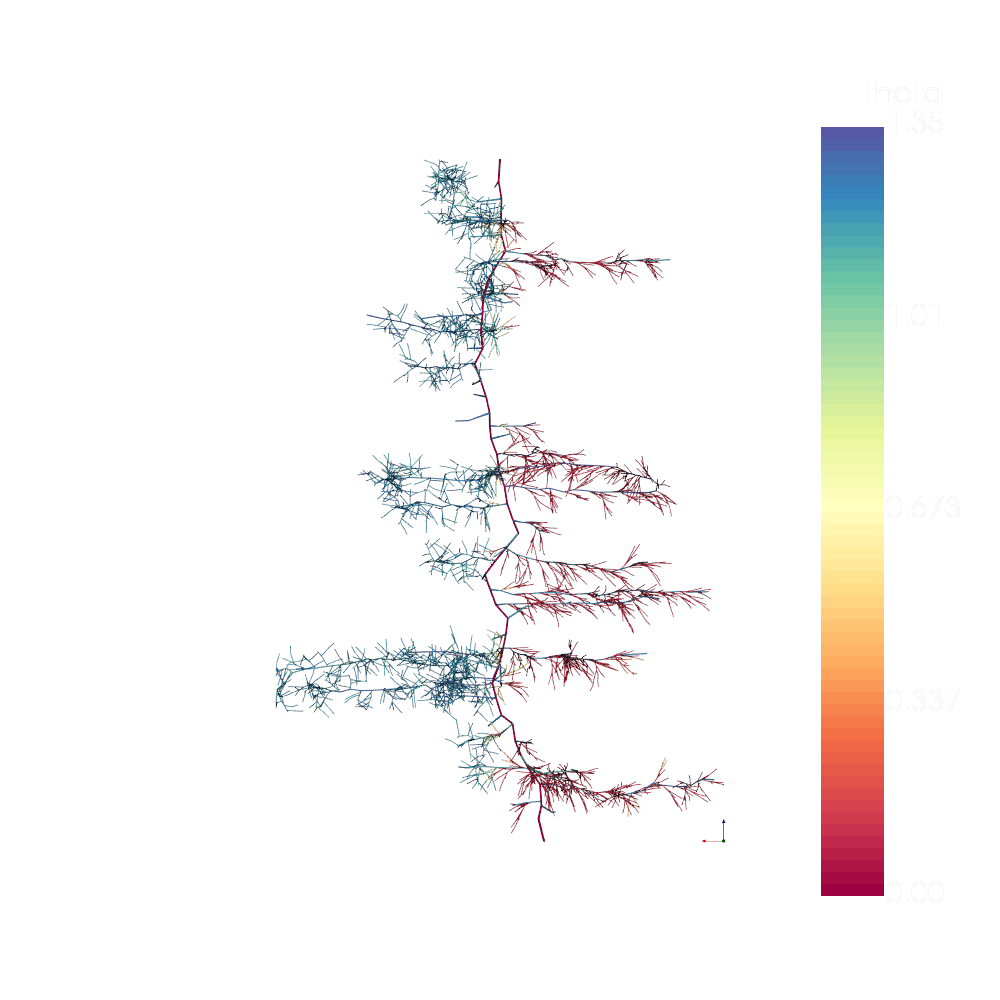
\includegraphics[width=0.5\textwidth]{example5c.png}
\caption{Insertion angle} \label{fig:insertion}
\end{figure}


\subsection{Change of lateral emergence probability} \label{sec:branching}

Soil properties can affect branching patterns. In the following example two compartments are created ( analog to Example 5a), and the branching probability is modified in each of them.

\lstinputlisting[firstline=1, language=Python, caption=Example 5d]{../../examples/python/example5d_branching.py}

\begin{itemize}

\item[27-30] Adjusts axial resolution and tortuosity.

\item[33, 34] We adjust the inter lateral distances by making it smaller for a factor five.

\item[35, 36] We set the branching probability scaling for the second order laterals. The scaling value means the probability that the branch occurs per day, i.e. 1 means the laterals always emerge (left compartment), or that they emerge with a chance of 0.2 \% per day (right compartment). 

\item[46-54] Analysis the root insertion angle in the left and right compartment. 

\item[61] A vtk simulation of root lengths. Press 'y' to obtain a x-z view of the root system to better see the effect (see Figure \ref{fig:probability}). 

\end{itemize}

Note that a scaling of zero means, that the laterals do never emerge, one means they always do. While the branching probability model is limited, it is easy to modify it to implement plant systemic responses. For this a suitable SoilLookUP must be defined and the method getValue(x, organ) must be overwritten, implementing the plant control of the branching probabilities. 

\begin{figure}
\centering
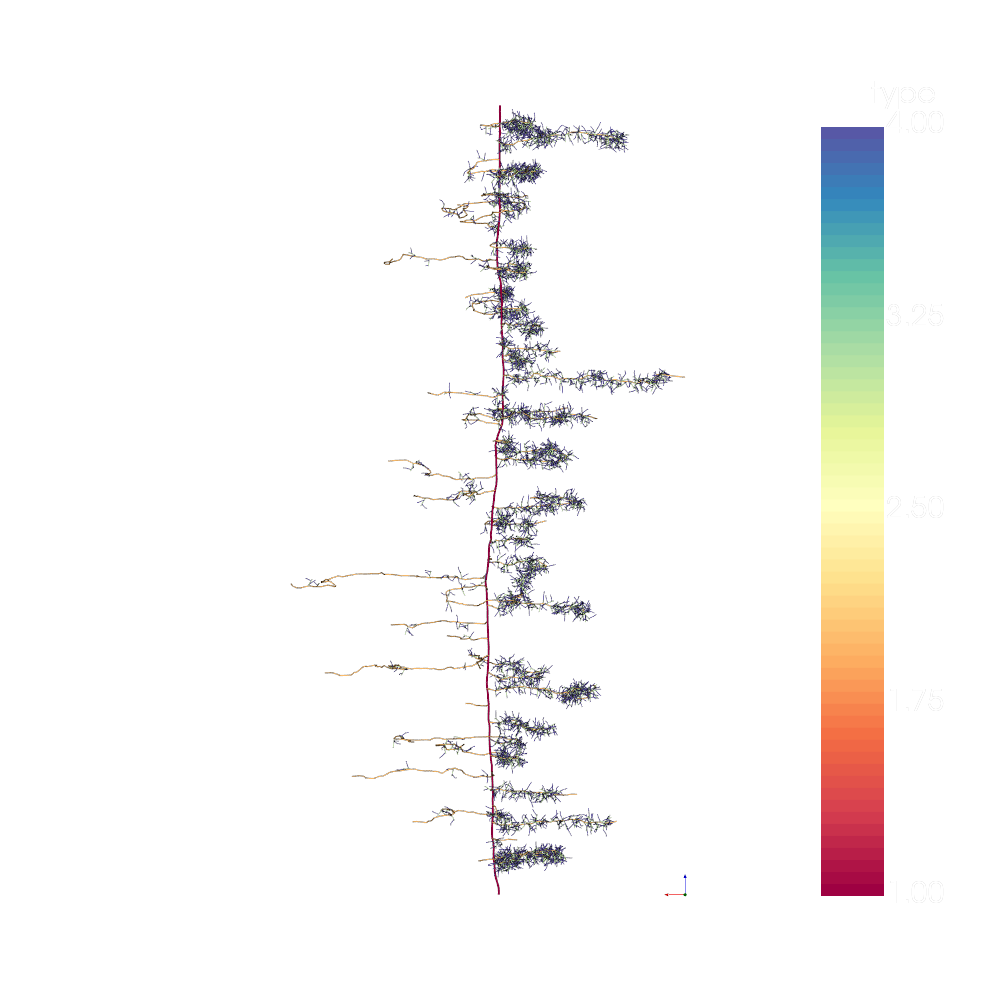
\includegraphics[width=0.5\textwidth]{example5d.png}
\caption{Branching density (probabilistic model)} \label{fig:probability}
\end{figure}
